%!TEX root = ../../thesis.tex

\subsection{Luminosity measurement}



\subsection{Run I dataset}

The recording of proton-proton collisions during run I of the LHC has been incredibly 
successful. In 2010, an integrated luminosity of \unit{45}{\invpb} was recorded at a 
centre-of-mass energy \unit{$\sqrt{s} = 7$}{\TeV}. However, this data was not used in the 
analysis and will not be referred to later.

\begin{figure}
	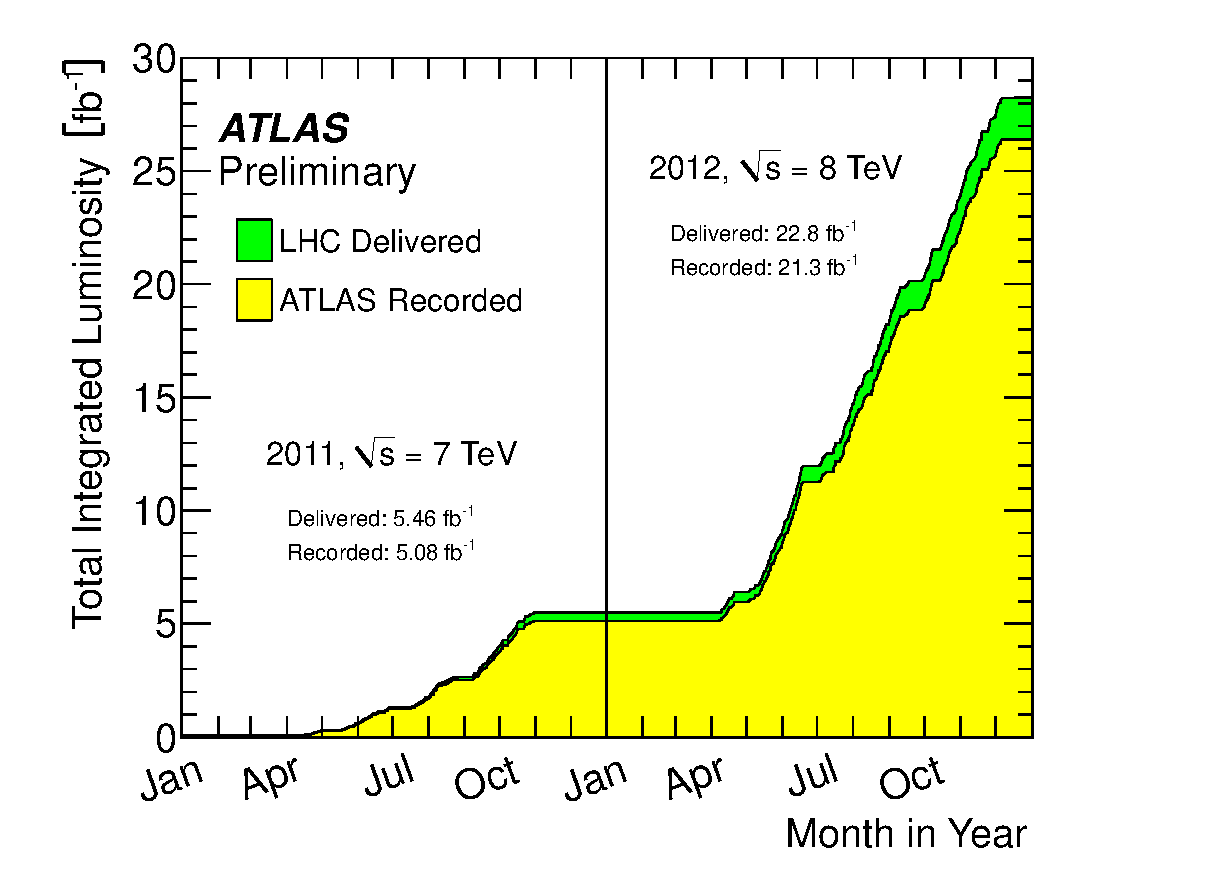
\includegraphics[width=\largefigwidth]{tex/experiment/luminosity}
	\caption{The cumulative luminosity delivered to (green) and recorded by (yellow) the
	ATLAS detector during run I of the \ac{LHC}. Differences reflect inefficiencies in the
	data acquisition. 
	\todo[inline]{Find reference, and check up-to-date}}
	\label{fig:luminosity}
\end{figure}

\begin{figure}
	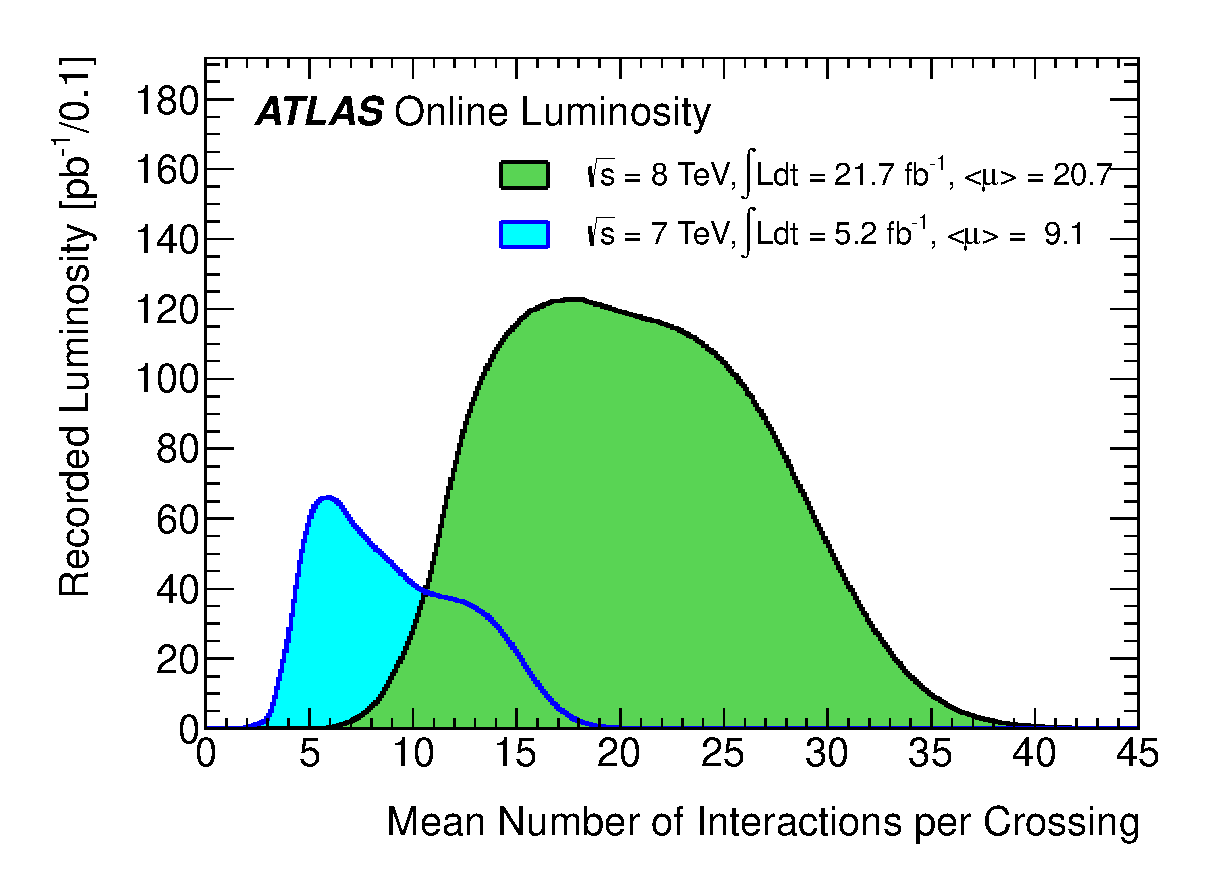
\includegraphics[width=\largefigwidth]{tex/experiment/pileup}
	\caption{The mean number of interactions per bunch crossing, $\mu$, for the 2011 (blue)
	and 2012 (green) datasets. These were calculated with an inelastic scattering cross 
	section of \unit{71.5}{\milli\barn} at \unit{$\sqrt{s} = 7$}{\TeV} and 
	\unit{73.0}{\milli\barn} at \unit{$\sqrt{s} = 8$}{\TeV}.}
	\label{fig:pileup}
\end{figure}

